%%%%%%%%%%%%%%%%%
% This is an example CV created using altacv.cls (v1.1, 21 November 2016) written by
% LianTze Lim (liantze@gmail.com), based on the 
% Cv created by BusinessInsider at http://www.businessinsider.my/a-sample-resume-for-marissa-mayer-2016-7/?r=US&IR=T
% 
%% It may be distributed and/or modified under the
%% conditions of the LaTeX Project Public License, either version 1.3
%% of this license or (at your option) any later version.
%% The latest version of this license is in
%%    http://www.latex-project.org/lppl.txt
%% and version 1.3 or later is part of all distributions of LaTeX
%% version 2003/12/01 or later.
%%%%%%%%%%%%%%%%

%% If you want to use \orcid or the
%% academicons icons, add "academicons"
%% to the \documentclass options. 
%% Then compile with XeLaTeX or LuaLaTeX.
% \documentclass[10pt,a4paper,academicons]{altacv}
\documentclass[10pt,a4paper]{altacv}

%% AltaCV uses the fontawesome and academicon fonts
%% and packages. 
%% See texdoc.net/pkg/fontawecome and http://texdoc.net/pkg/academicons for full list of symbols.
%% When using the "academicons" option,
%% Compile with LuaLaTeX for best results. If you
%% want to use XeLaTeX, you may need to install
%% Academicons.ttf in your operating system's font %% folder.


% Full-width geometry for page 1
\geometry{left=1cm,right=1cm,top=1cm,bottom=1cm}
% Save two-column geometry for page 2
\newcommand{\twocolgeometry}{\newgeometry{left=1cm,right=9cm,marginparwidth=6.8cm,marginparsep=1.2cm,top=1cm,bottom=1cm}}

% Change the font if you want to.

% If using pdflatex:
\usepackage[utf8]{inputenc}
\usepackage[T1]{fontenc}
\usepackage[default]{lato}
\usepackage{enumitem} % For customizing lists
\usepackage{multicol} % For multi-column layout
\usepackage{ragged2e} % For text justification
\usepackage{pgfplots} % For bar charts
\pgfplotsset{compat=1.17}
% Colors for bar chart (blue-green palette)
\definecolor{colorB2B}{HTML}{1A5276}
\definecolor{colorProspeccion}{HTML}{1E8C8C}
\definecolor{colorCRM}{HTML}{48B4A0}
\definecolor{colorCierre}{HTML}{6BC9A6}
\definecolor{colorDificultades}{HTML}{8FD9B6}
\definecolor{colorPruebas}{HTML}{B5E7A0}

% Colors for wheelchart (blue-teal palette)
\definecolor{wheel1}{HTML}{1B4F72}
\definecolor{wheel2}{HTML}{2874A6}
\definecolor{wheel3}{HTML}{1ABC9C}
\definecolor{wheel4}{HTML}{48C9B0}
\definecolor{wheel5}{HTML}{76D7C4}
\definecolor{wheel6}{HTML}{A3E4D7}

% If using xelatex or lualatex:
% \setmainfont{Lato}

% Change the colours if you want to
\definecolor{VividPurple}{HTML}{1B4A5C}
\definecolor{SlateGrey}{HTML}{2E2E2E}
\definecolor{LightGrey}{HTML}{666666}
\colorlet{heading}{VividPurple}
\colorlet{accent}{VividPurple}
\colorlet{emphasis}{SlateGrey}
\colorlet{body}{LightGrey}

% Change the bullets for itemize and rating marker
% for \cvskill if you want to
\renewcommand{\itemmarker}{{\small\textbullet}}
\renewcommand{\ratingmarker}{\faCircle}

%% sample.bib contains your publications
% \addbibresource{sample.bib} % Commented out - publications not used

% Redefine cvevent so date and location are closer together
\renewcommand{\cvevent}[4]{%
  {\large\bfseries\color{emphasis}#1\par}
  \smallskip
  \textbf{\color{accent}#2}\par
  \smallskip
  {\small\faCalendar \hspace{0.5em}#3\hspace{2em}%
  \ifstrequal{#4}{}{}{\faMapMarker\hspace{0.5em}#4}\par}
  \medskip
}

% Redefine wheelchart without centering for manual positioning
\renewcommand{\wheelchart}[3]{%
    \begingroup
    \def\innerradius{#2}%
    \def\outerradius{#1}%
    \pgfmathsetmacro{\totalnum}{0}%
    \foreach \value/\colour/\name in {#3} {%
        \pgfmathparse{\value+\totalnum}%
        \global\let\totalnum=\pgfmathresult%
    }%
    \begin{tikzpicture}
      \pgfmathsetmacro{\wheelwidth}{\outerradius-\innerradius}
      \pgfmathsetmacro{\midradius}{(\outerradius+\innerradius)/2}
      \begin{scope}[rotate=-90]
      \pgfmathsetmacro{\cumnum}{0}
      \foreach \value/\width/\colour/\name in {#3} {
            \pgfmathsetmacro{\newcumnum}{\cumnum + \value/\totalnum*360}
            \pgfmathsetmacro{\percentage}{\value/\totalnum*100}
            \pgfmathsetmacro{\midangle}{-(\cumnum+\newcumnum)/2}
            \pgfmathparse{(-\midangle>180?"west":"east")} \edef\textanchor{\pgfmathresult}
            \pgfmathparse{(-\midangle>180?"flush left":"flush right")} \edef\textalign{\pgfmathresult}
            \pgfmathsetmacro\labelshiftdir{1-2*(-\midangle<180)}
            \filldraw[draw=white,fill=\colour] (-\cumnum:\outerradius) arc (-\cumnum:-(\newcumnum):\outerradius) --
            (-\newcumnum:\innerradius) arc (-\newcumnum:-(\cumnum):\innerradius) -- cycle;
            \draw [*-,thin,emphasis] node [append after command={(\midangle:\midradius pt) -- (\midangle:\outerradius + 1ex) -- (\tikzlastnode)}] at (\midangle:\outerradius + 1ex) [xshift=\labelshiftdir*0.5cm,inner sep=1ex, outer sep=0pt, text width=\width,anchor=\textanchor,align=\textalign,font=\small,text=body]{\name};
            \global\let\cumnum=\newcumnum
        }
      \end{scope}
    \end{tikzpicture}\par
    \endgroup
}

\begin{document}
\name{Ana María \newline Albarracín Noreña}
  \tagline{B2B Sales Executive}
% Cropped to square from https://en.wikipedia.org/wiki/Marissa_Mayer#/media/File:Marissa_Mayer_May_2014_(cropped).jpg, CC-BY 2.0
\photo{5.5cm}{me}
% Personal info without bullet points
\personalinfo{%
  \textcolor{accent}{\faEnvelope}\hspace{0.5em}amalbarracin5@gmail.com \\
  \textcolor{accent}{\faPhone}\hspace{0.5em}(+57) 312 825 5775 \\
  \textcolor{accent}{\faLinkedin}\hspace{0.5em}linkedin.com/in/ana-maria-albarracin \\
  \textcolor{accent}{\faMapMarker}\hspace{0.5em}Professional card: 26272
}

\makecvheader

\cvsection{Sales Skills}
\begin{center}
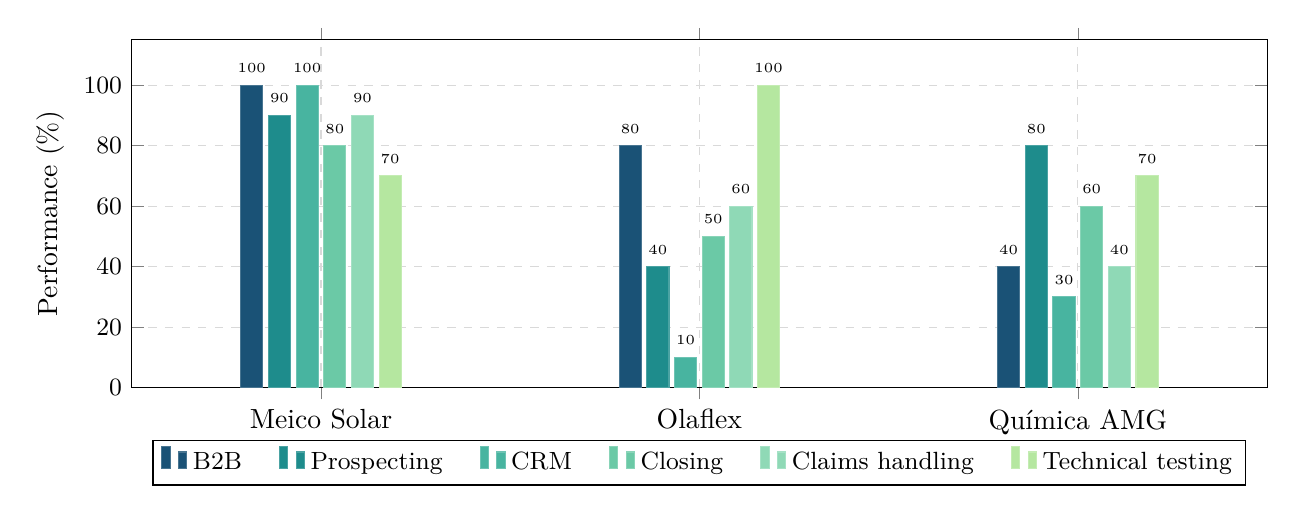
\begin{tikzpicture}
\begin{axis}[
    ybar,
    width=16cm,
    height=6cm,
    bar width=8pt,
    ylabel={Performance (\%)},
    ymin=0,
    ymax=115,
    ytick={0,20,40,60,80,100},
    symbolic x coords={Meico Solar, Olaflex, Química AMG},
    xtick=data,
    x tick label style={font=\normalsize},
    y tick label style={font=\small},
    ylabel style={font=\normalsize},
    legend style={
        at={(0.5,-0.15)},
        anchor=north,
        legend columns=6,
        font=\small,
        /tikz/every even column/.append style={column sep=0.4cm}
    },
    nodes near coords,
    nodes near coords style={font=\tiny, above},
    every node near coord/.append style={yshift=1pt},
    enlarge x limits=0.25,
    grid=major,
    grid style={dashed, gray!30},
]
% B2B - Dark blue
\addplot[fill=colorB2B, draw=colorB2B!80] coordinates {
    (Meico Solar,100) (Olaflex,80) (Química AMG,40)
};
% Prospecting
\addplot[fill=colorProspeccion, draw=colorProspeccion!80] coordinates {
    (Meico Solar,90) (Olaflex,40) (Química AMG,80)
};
% CRM
\addplot[fill=colorCRM, draw=colorCRM!80] coordinates {
    (Meico Solar,100) (Olaflex,10) (Química AMG,30)
};
% Closing
\addplot[fill=colorCierre, draw=colorCierre!80] coordinates {
    (Meico Solar,80) (Olaflex,50) (Química AMG,60)
};
% Claims handling
\addplot[fill=colorDificultades, draw=colorDificultades!80] coordinates {
    (Meico Solar,90) (Olaflex,60) (Química AMG,40)
};
% Technical testing
\addplot[fill=colorPruebas, draw=colorPruebas!80] coordinates {
    (Meico Solar,70) (Olaflex,100) (Química AMG,70)
};
\legend{B2B, Prospecting, CRM, Closing, Claims handling, Technical testing}
\end{axis}
\end{tikzpicture}
\end{center}

\vspace{0.3cm}
\begin{multicols}{2}
\small
\textbf{\color{accent}B2B}\\
Negotiation with companies.\\[4pt]
\textbf{\color{accent}Prospecting}\\
Search, contact, company presentation and qualification of potential clients.\\[4pt]
\textbf{\color{accent}CRM}\\
Business logging, timely follow-up and sales process management.

\columnbreak

\textbf{\color{accent}Closing}\\
Final negotiation and effective sales closing.\\[4pt]
\textbf{\color{accent}Claims handling}\\
Management of dissatisfied customers and incidents.\\[4pt]
\textbf{\color{accent}Technical testing}\\
Staff training and performance testing of materials in different production environments.
\end{multicols}

\cvsection{Work Experience}
\cvevent{Senior Sales Executive - Line Specialist}{Meico Solar}{May 2024--Present}{Bogotá, Colombia}
{\color{accent}\textbf{Sales Executive}}
\begin{itemize}
\item Full commercial management: prospecting, needs identification, quoting, strategic follow-up and sales closing with post-sales support.
\item Relationship visits in Bogotá and the Coffee Region to strengthen ties with current and potential clients.
\item Search for new business opportunities based on analysis of large client sector data, with structured follow-up and approach strategy proposals.
\item Market analysis and CRM maintenance to identify opportunities.
\end{itemize}

{\color{accent}\textbf{Promotion: Senior Sales Executive - Line Specialist}} {\small\textit{(October 2025)}}
\begin{itemize}
\item Key account management and leadership in strategic product line negotiations.
\item Training and mentoring of the sales team; line budget follow-up and control.
\item Design of commercial strategies: marketing campaigns, webinars and support in forecast and deal closing.
\end{itemize}

\cvevent{Technical Sales Advisor}{Olaflex SAS}{July 2022--May 2024}{Bogotá, Colombia}

\begin{itemize}
\item Polyurethane product sales management, including client visits and follow-up.
\item Proposal of custom developments according to end-use, including plant technical support, performance testing and formulation of customized solutions.
\item Development of marketing plans and budget projections.
\item Export coordination, legal and customs documentation handling.
\end{itemize}
\vspace{0.2 cm}
\cvevent{Sales Advisor}{Química MG}{January 2022--July 2022}{Bogotá, Colombia}

\begin{itemize}
\item Participation in tenders and engineering projects.
\item Preparation of commercial proposals and client follow-up.
\end{itemize}

\cvevent{Project Manager}{Grupo Coral SAS}{January 2020--August 2021}{Bogotá, Colombia}

\begin{itemize}
\item Preparation of technical-commercial proposals for public and private sector clients.
\item Support in tender processes and new business development.
\end{itemize}

% Start of two-column section
\begin{multicols}{2}

\cvsection{What information do I obtain in a sales meeting?}
{\small\justifying In a meeting with the client, through the right questions, I identify the following key information:\par}
\vspace{0.2cm}
\noindent\makebox[\columnwidth][l]{%
\hspace{-3cm}\wheelchart{2.5cm}{0.5cm}{%
30/12em/wheel1/Business\\knowledge,
25/12em/wheel2/Client\\knowledge,
20/10em/wheel3/Competition,
15/12em/wheel4/Commercial\\proposal,
10/12em/wheel5/Negotiation\\status}}

\vspace{0.3cm}
{\small\justifying
\textbf{\color{accent}Business knowledge:} Times, internal processes and products.\\[2pt]
\textbf{\color{accent}Client knowledge:} Key roles and decision makers.\\[2pt]
\textbf{\color{accent}Competition:} Competitors, prices and value propositions.\\[2pt]
\textbf{\color{accent}Negotiation status:} Current prices and commercial conditions.\\[2pt]
\textbf{\color{accent}Commercial proposal:} Technical info, prices and value arguments.\par
}

\cvsection{Languages}
\cvskill{Spanish}{5}
\divider
\cvskill{English}{3}

\cvsection{References}
\cvref{Daniela Perdomo Morales, Sales Executive, Biopolar}{+57 313 8653659}{}
\divider
\cvref{Juan David Tuta Botero, Engineering Lead, Unosquare}{+57 3016395759}{}

\columnbreak

% \vspace*{0.0003cm}
\cvsection{Education}
\cvevent{Master's in Chemical Engineering}{Universidad Nacional de Colombia}{2023--Present}{Bogotá, Colombia}
{\justifying Thesis in progress: Comparison of multicriteria methods for the selection of CO capture and application technologies in high-emission industries. The project integrates technologies such as amine absorption, membranes and solid adsorption, evaluated through tools such as AHP, TOPSIS and Fuzzy TOPSIS.\par}

\cvevent{Chemical Engineering}{Universidad Nacional de Colombia}{2013--2019}{Bogotá, Colombia}
{\justifying Thesis: Comparison of catalysts for plasma hydrolysis for food purposes. Solid training in chemical processes, quality control and physicochemical analysis. Developed practical experience in the fragrance industry, including sampling, SAP and batch release.\par}

\cvsection{Interests}
\cvachievement{\faBook}{Professional Development}{Reading on sales trends, industrial sustainability and new energy technologies.}
\cvachievement{\faHeart}{Personal Development}{Meditation practice, emotional management, creativity development and constant pursuit of new experiences.}
\cvachievement{\faUsers}{Networking}{Participation in sales events, industrial fairs and professional communities.}

\end{multicols}

\end{document}
